\documentclass[aspectratio=169]{beamer}
\usetheme{Boadilla}



\usepackage[utf8]{inputenc}       % Codificação de entrada
\usepackage[T1]{fontenc}          % Codificação de saída
\usepackage[portuguese]{babel}   % Idioma
\usepackage{XCharter}             % Fonte principal
\AtBeginDocument{\fontsize{12}{12}\selectfont}

%\usepackage{geometry}
%\geometry{papersize={210mm,150mm}}

\usepackage{color}
\usepackage{graphicx}
\usepackage{amsmath, amssymb, amsfonts}
\usepackage{bm}
\usepackage{booktabs}
\usepackage{multirow}
\usepackage{caption}
\usepackage{subfigure}
\usepackage{wrapfig}
\usepackage{multicol}
\usepackage{sidecap}
\usepackage{tikz}
\usepackage{listings}
\usepackage{siunitx}
\usepackage{pdfpages}
\usepackage{float}
\usepackage{hyperref}
\usepackage{academicons}
\usepackage{setspace}

\newcommand{\eng}[1]{\textsl{#1}}
\newcommand{\cod}[1]{\texttt{#1}}


\title[Minicurso FPGAs]{\huge Introdução ao VHDL}


\author[Prof. Dr. Oscar Eduardo Anacona Mosquera]{Prof. Dr. Oscar Eduardo Anacona Mosquera \newline\newline 
\scriptsize{oscar.mosquera@ufmt.br}
}


\AtBeginSection[]
{
	\begin{frame}{Conteúdo}
		\tableofcontents[currentsection]
	\end{frame}
}


\begin{document}

\begin{frame}[plain]
\titlepage
%\vspace{3cm}
%\begin{center} \color{MULTurquoise} {Chair of Cyber-Physical-Systems}\end{center}

\end{frame}


\section{Objetivos}

%%====================================================================================
%%====================================================================================
\begin{frame}
	\frametitle{Objetivos}
	
	\begin{itemize}
		\justifying
		\item \textbf{Introdução à VHDL:}
		\begin{itemize}
			\justifying
			\item Compreender os fundamentos da VHDL como uma linguagem de descrição de hardware.
			%\item Explorar a evolução do fluxo de projeto em VHDL, desde suas origens até os métodos modernos.
		\end{itemize}
		
		\item \textbf{Modelo de um Arquivo VHDL: Composição e Estrutura:}
		\begin{itemize}
			\justifying
			\item Analisar a estrutura de um arquivo VHDL, incluindo entidades, arquiteturas e bibliotecas.
			%\item Compreender a composição de um modelo VHDL e sua importância no design de circuitos digitais.
		\end{itemize}
		
		\item \textbf{Declarações Concorrentes em VHDL:}
		\begin{itemize}
			\justifying
			\item Explorar declarações concorrentes em VHDL, como processos, blocos e sinais.
			%\item Compreender como as declarações concorrentes são usadas para descrever comportamentos simultâneos em circuitos digitais.
		\end{itemize}
		
		\item \textbf{Declarações Sequenciais em VHDL:}
		\begin{itemize}
			\justifying
			\item Analisar declarações sequenciais em VHDL, como o uso dos Flip-Flops.
			%\item Entender como as declarações sequenciais são usadas para descrever comportamentos que ocorrem em uma sequência específica.
		\end{itemize}
		
		\item \textbf{Máquinas de Estados Finitas em VHDL:}
		\begin{itemize}
			\justifying
			\item Compreender os princípios fundamentais das máquinas de estados finitas (FSMs).
			%\item Desenvolver habilidades para implementar FSMs em VHDL para sistemas sequenciais.
		\end{itemize}	
		
	\end{itemize}
\end{frame}
%%====================================================================================
%%====================================================================================
\section{Linguagem de descrição de hardware VHDL}
%%====================================================================================
%%====================================================================================
\begin{frame}{VHDL}
	\justifying
	
	\begin{block}{}
		\justifying
		A VHDL permite que os engenheiros descrevam o comportamento e a estrutura de circuitos digitais complexos. Essa descrição pode incluir informações sobre sinais, portas, componentes, processos, temporização e outros aspectos do projeto.
	\end{block}
	
	\begin{itemize}
		\item \textbf{V}HSIC (Very High Speed Integrated Circuit)
		\item \textbf{H}ardware
		\item \textbf{D}escription
		\item \textbf{L}anguage
	\end{itemize}
	
\begin{alertblock}{}
``\textbf{Tell me how your circuit should behave and I will give you
hardware that does the job.}”
\end{alertblock}	
	
	
\end{frame}
%%====================================================================================
%%====================================================================================

\begin{frame}{Principais características}
\justifying
	
	\begin{itemize}
		\justifying
		\item \textbf{Descrição de Hardware:} VHDL permite a descrição abstrata de sistemas digitais, abrangendo desde níveis mais altos de comportamento até detalhes de baixo nível.
		\item \textbf{Simulação e Verificação:} A linguagem é amplamente utilizada em simulação para verificar o comportamento e o desempenho dos projetos antes da implementação física.
		\item \textbf{Síntese Lógica:} VHDL é frequentemente utilizado em conjunto com ferramentas de síntese para transformar a descrição de alto nível em uma implementação específica em hardware.
		\item \textbf{Projeto de Circuitos Complexos:} É particularmente útil para projetar sistemas digitais complexos, como processadores, sistemas embarcados, e outros dispositivos eletrônicos.

	\end{itemize}
	
	
\end{frame}
%%====================================================================================
%%====================================================================================



\begin{frame}{Principais características}
	\justifying
	
	\begin{itemize}
		\justifying

		\item \textbf{Reutilização de Design:} A VHDL suporta a reutilização de design, permitindo que módulos e componentes sejam definidos e posteriormente utilizados em diferentes projetos
		\item \textbf{Padrão IEEE:} VHDL é um padrão IEEE (\textbf{Institute of Electrical and Electronics Engineers}), o que contribui para sua ampla aceitação e uso na indústria.
		\item \textbf{Síntese para FPGAs e ASICs:} Pode ser utilizado para a síntese de projetos em FPGAs ou ASICs, convertendo a descrição em hardware físico.
	\end{itemize}
	
	
\end{frame}

%%====================================================================================
%%====================================================================================

\begin{frame}{Terminologia}
	\justifying
	
	\begin{itemize}
		\justifying
		\item \textbf{HDL:} uma limguagem de descrição de hardware é uma linguagem de programação de software usada para a modelagem de um circuito hardware.
		
		\item \textbf{Modelo comportamental:} um componente é descrito pela resposta das entradas e saídas.
		
		\item \textbf{Modelo estrutural:} um componente é descrito pela interconexão de componentes/primitivas de níveis mais baixos (\textbf{abordagem top-down design}).
		
	\end{itemize}
	
	
\end{frame}
%%====================================================================================
%%====================================================================================

\begin{frame}{Modelo comportamental (Behavioral Modeling)}
	\justifying

	\begin{itemize}
	\justifying
	\item Somente a funcionalidade do circuito, não a estrutura.
	
	\item A descrição do hardware não está vinculada a uma implementação específica de hardware.

\end{itemize}

	
	\begin{figure}[h]
		\centering
		\includegraphics[width=0.67\textwidth]{Figs/fig03.png}
	\end{figure}
	
	
\end{frame}

%%====================================================================================
%%====================================================================================

\begin{frame}{Modelo estrutural (Structural Modeling)}
	\justifying
	
	\begin{itemize}
		\justifying
		\item Funcionalidade e estrutura do circuito.
	\end{itemize}
	
	
	\begin{figure}[h]
		\centering
		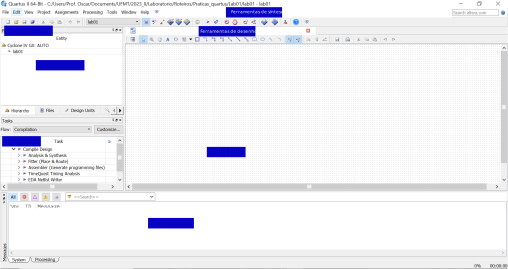
\includegraphics[width=0.67\textwidth]{Figs/fig04.png}
	\end{figure}
	
	
\end{frame}
%%====================================================================================
%%====================================================================================
\begin{frame}{Terminologia}
	\justifying
	
	\begin{itemize}
		\justifying
		\item \textbf{Register Transfer Level (RTL):} um tipo de modelo comportamental, com o propósito de síntese. O hardware é implícito e é sintetizável.
		
		\item \textbf{Síntese:} traduzindo HDL para um circuito e, em seguida, otimizando o circuito representado.
		
		\item \textbf{Processo:} unidade básica de execução em VHDL (são convertidos para seu equivalente em hardware).
		
		
	\end{itemize}
	
	
\end{frame}
%%====================================================================================
%%====================================================================================
\begin{frame}{RTL Synthesis}
	\justifying
	
	
	\begin{figure}[h]
		\centering
		\includegraphics[width=0.75\textwidth]{Figs/fig05.png}
	\end{figure}
	
	
\end{frame}
%%====================================================================================
%%====================================================================================
\begin{frame}{Translation of VHDL Code into a Circuit}
	\justifying
	
	
	\begin{figure}[h]
		\centering
		\includegraphics[width=0.5\textwidth]{Figs/fig93.png}
	\end{figure}
	
	
\end{frame}
%%====================================================================================
%%====================================================================================
\begin{frame}{VDHL básico}
	\justifying
	
	\begin{itemize}
		\justifying
		\item A linguagem VHDL é composta por palavras-chave reservadas.
		
		\item A linguagem, em sua maior parte, não é sensível a maiúsculas e minúsculas.
		
		\item As declarações VHDL são terminadas com um ponto e vírgula, ``;".
		
		\item VHDL é insensível a espaços em branco.
		
		\item \textbf{-- : Comentário de fim de linha (EOL)}; tudo a partir do símbolo até o EOL é comentado.
		
		\item \textbf{/* */} : Comentário delimitado; tudo entre os símbolos é comentado.
	\end{itemize}
	
	
\end{frame}
%%====================================================================================
%%====================================================================================
\begin{frame}{Palavras chave}
	\justifying
	
	
	\begin{figure}[h]
		\centering
		\includegraphics[width=0.5\textwidth]{Figs/fig27.png}
	\end{figure}
	
	
\end{frame}
%%====================================================================================
%%====================================================================================
\begin{frame}{Unidades de Design VHDL}
	\justifying
	
	\begin{itemize}
		\justifying
		\item \textbf{Entidades (Entities):} Entidades definem a interface do componente, especificando seus sinais de entrada e saída. Elas são como um contrato que descreve o comportamento externo do componente. As entidades não contêm lógica interna.
		
		\item \textbf{Arquiteturas (Architectures):} Arquiteturas definem a lógica interna de uma entidade. Elas descrevem como os sinais de entrada são manipulados para produzir os sinais de saída. Uma entidade pode ter várias arquiteturas, cada uma representando uma implementação diferente.
		
		\item \textbf{Pacotes (Packages):} Pacotes são usados para agrupar constantes, tipos de dados, subprogramas e outras declarações que podem ser compartilhadas entre várias entidades e arquiteturas. Eles são úteis para promover a reutilização e a organização do código.
		
		

	\end{itemize}
	
	
\end{frame}

%%====================================================================================
%%====================================================================================
\begin{frame}{Unidades de Design VHDL}
	\justifying
	
	\begin{itemize}
		\justifying

		
		\item \textbf{Configurações (Configurations):} Configurações são usadas para associar uma entidade a uma arquitetura específica ou a outras entidades. Elas permitem configurar a hierarquia do projeto e selecionar as implementações desejadas para cada componente.
		
		\item \textbf{Bibliotecas (Libraries):} Bibliotecas são coleções de unidades de design relacionadas, como entidades, arquiteturas e pacotes. Elas ajudam a organizar e gerenciar o código, permitindo a reutilização de unidades em diferentes projetos.
		
		
	\end{itemize}
	
	
\end{frame}

%%====================================================================================
%%====================================================================================
\begin{frame}{Unidades de Design VHDL}
	\justifying
	
	
	\begin{figure}[h]
		\centering
		\includegraphics[width=0.7\textwidth]{Figs/fig10.png}
	\end{figure}
	
	
\end{frame}
%%====================================================================================
%%====================================================================================
\begin{frame}{Declaração da Entidade}
	\justifying
	
	
	\begin{figure}[h]
		\centering
		\includegraphics[width=1\textwidth]{Figs/fig09.png}
	\end{figure}
	
	
\end{frame}
%%====================================================================================
%%====================================================================================
\begin{frame}{Declaração da Entidade}
	\justifying
	
	
	\begin{figure}[h]
		\centering
		\includegraphics[width=0.97\textwidth]{Figs/fig11.png}
	\end{figure}
	
	
\end{frame}
%%====================================================================================
%%====================================================================================
\begin{frame}{Declaração da Entidade}
	\justifying
	
	Há quatro modos possíveis de uma porta, são eles:
	
	\begin{itemize}
		\item \textbf{IN:} porta de entrada.
		\item \textbf{OUT:} porta de saída, não pode ser referenciado internamente pela arquitetura.
		\item \textbf{BUFFER:} a porta opera unicamente no modo saída, pode ser referenciado internamente pela arquitetura.
		\item \textbf{INOUT:} caracteriza uma porta bidirecional onde uma informação pode ser apresentada ou amostrada.
	\end{itemize}
	
	
	
\end{frame}
%%====================================================================================
%%====================================================================================
\begin{frame}{Corpo da arquitetura}
	\justifying
	
	
	\begin{block}{}
	\justifying
	A ``ARCHITECTURE" em VHDL é usada para definir o comportamento ou a estrutura interna de um componente digital descrito na linguagem. 
	
	\begin{itemize}
	\item Descreve a funcionalidade.
	\item Declarações são executadas concorrentemente (processos).
	\item Podem ser colocadas várias arquiteturas.
	\item \textbf{Behavioral:} mostra como funciona.
	\item \textbf{RTL:} A descrição dos designs é feita em termos de registradores.
	\item \textbf{Hybrid:} mistura de ambos estilos.
	\end{itemize}	
	
	\end{block}	
	
\end{frame}

%%====================================================================================
%%====================================================================================

\begin{frame}{Corpo da arquitetura}
	\justifying
	
	\begin{figure}[h]
		\centering
		\includegraphics[width=0.97\textwidth]{Figs/fig14.png}
	\end{figure}

\end{frame}

%%====================================================================================
%%====================================================================================

\begin{frame}{Corpo da arquitetura}
	\justifying
	
	
	\begin{figure}[h]
		\centering
		\includegraphics[width=0.97\textwidth]{Figs/fig29.png}
	\end{figure}
	
	
	
\end{frame}
%%====================================================================================
%%====================================================================================
\begin{frame}{Corpo da arquitetura}
	\justifying
	
	
	\begin{figure}[h]
		\centering
		\includegraphics[width=0.97\textwidth]{Figs/fig15.png}
	\end{figure}
	
	
	
\end{frame}
%%====================================================================================
%%====================================================================================
\begin{frame}{VHDL- Estrutura Básica de Modelagem}
	\justifying
	
	
	\begin{figure}[h]
		\centering
		\includegraphics[width=0.77\textwidth]{Figs/fig16.png}
	\end{figure}
	
	
	
\end{frame}
%%====================================================================================
%%====================================================================================
\begin{frame}{Tipos de dados}
	\justifying

	\begin{figure}[h]
		\centering
		\includegraphics[width=0.97\textwidth]{Figs/fig21.png}
	\end{figure}

\end{frame}
%%====================================================================================
%%====================================================================================
\begin{frame}{Tipos de dados}
	\justifying
	
	
	\begin{figure}[h]
		\centering
		\includegraphics[width=0.9\textwidth]{Figs/fig22.png}
	\end{figure}	
	
\end{frame}
%%====================================================================================
%%====================================================================================
\begin{frame}{VHDL- pacotes std e IEEE}
	\justifying
	

	
	\begin{figure}[h]
		\centering
		\includegraphics[width=0.7\textwidth]{Figs/fig28.png}
	\end{figure}	
	
\end{frame}
%%====================================================================================
%%====================================================================================
\begin{frame}{VHDL- pacotes std e IEEE: tipos sintetizáveis}
	\justifying
	
	
	
	\begin{figure}[h]
		\centering
		\includegraphics[width=0.65\textwidth]{Figs/fig36.png}
	\end{figure}	
	
\end{frame}

%%====================================================================================
%%====================================================================================

\begin{frame}{VHDL- pacotes std e IEEE}
	\justifying
	
	\begin{block}{Type STD$\_$LOGIC}
		9 logic value system (‘U’, ‘X’, ‘0’, ‘1’, ‘Z’, ‘W’, ‘L’, ‘H’, ‘-’)
		
	\begin{itemize}
	\item \textbf{1:} Logic high    
	\item \textbf{0:} Logic low
	\item \textbf{X:} Unknown
	\item \textbf{Z:} (not ‘z’) Tri-state
	\item \textbf{-:} Don’t Care
	\item \textbf{U:} Undefined
	\item \textbf{H:} Weak logic high
	\item \textbf{L:} Weak logic low
	\item \textbf{W:} Weak unknown
	\end{itemize}		
		
		
	\end{block}

	
\end{frame}
%%====================================================================================
%%====================================================================================
\begin{frame}{Conversão de tipos de dados}
	\justifying
	
	
	
	\begin{figure}[h]
		\centering
		\includegraphics[width=0.45\textwidth]{Figs/vhdl-type-conversions.png}
	\end{figure}	
	
\end{frame}
%%====================================================================================
%%====================================================================================
\begin{frame}{Definição de novos tipos}
	\justifying
	
	\begin{block}{}
	\justifying
	A linguagem VHDL permite a criação de novos tipos enumerados, físicos e compostos.
	\end{block}		
	
	\begin{figure}[h]
		\centering
		\includegraphics[width=0.97\textwidth]{Figs/fig23.png}
	\end{figure}
	
\end{frame}

%%====================================================================================
%%====================================================================================
\begin{frame}{Definição de novos tipos}
	\justifying
	
	\begin{block}{Subtype}
		\justifying
		Sintetizável se o tipo base é sintetizável.
	\end{block}		
	
	\begin{figure}[h]
		\centering
		\includegraphics[width=0.57\textwidth]{Figs/fig73.png}
	\end{figure}
	
\end{frame}
%%====================================================================================
%%====================================================================================
\begin{frame}{Operadores}
	\justifying
	
	\begin{block}{}
		\justifying
		Os operadores definidos são divididos em classes que estabelecem a precedência na execução das operações.
	\end{block}		
	
	\begin{figure}[h]
		\centering
		\includegraphics[width=0.9\textwidth]{Figs/fig24.png}
	\end{figure}
	
	
\end{frame}
%%====================================================================================
%%====================================================================================
\begin{frame}{Operadores}
	\justifying
	
	
	\begin{figure}[h]
		\centering
		\includegraphics[width=0.9\textwidth]{Figs/fig25.png}
	\end{figure}
	
	
\end{frame}
%%====================================================================================
%%====================================================================================
\begin{frame}{Operadores}
	\justifying
	
	
	\begin{figure}[h]
		\centering
		\includegraphics[width=0.9\textwidth]{Figs/fig26.png}
	\end{figure}
	
	
\end{frame}
%%====================================================================================
%%====================================================================================
\begin{frame}{Operadores}
	\justifying
	
	
	\begin{figure}[h]
		\centering
		\includegraphics[width=0.77\textwidth]{Figs/fig30.png}
	\end{figure}
	
	
\end{frame}
%%====================================================================================
%%====================================================================================
\begin{frame}{Operadores: sinais usadas como interligação}
	\justifying
	
	
	\begin{figure}[h]
		\centering
		\includegraphics[width=0.77\textwidth]{Figs/fig32.png}
	\end{figure}
	
	
\end{frame}
%%====================================================================================
%%====================================================================================
\begin{frame}{Operadores: função aritmética}
	\justifying
	
	
	\begin{figure}[h]
		\centering
		\includegraphics[width=0.77\textwidth]{Figs/fig33.png}
	\end{figure}
	
	
\end{frame}
%%====================================================================================
%%====================================================================================
\begin{frame}{Exemplo}
	\justifying
	
	
	\begin{figure}[h]
		\centering
		\includegraphics[width=0.77\textwidth]{Figs/fig37.png}
	\end{figure}
	
	
\end{frame}
%%====================================================================================
%%====================================================================================
\section{Declarações Concorrentes}
%%====================================================================================
%%====================================================================================
\begin{frame}{Declarações Concorrentes}
	\justifying
	
	\begin{itemize}
		\item Declaração \textbf{when}
		\item Declaração \textbf{select}
		\item Declaração \textbf{generate}
		\item Declaração \textbf{Process}
	\end{itemize}
	
	
	\begin{block}{Declarações concorrentes}
	VHDL é inerentemente concorrente em vez de sequencial.	
		
	\end{block}
	
	
\end{frame}
%%====================================================================================
%%====================================================================================

\begin{frame}{Declarações Concorrentes}
	\justifying
	
	\begin{figure}[h]
		\centering
		\includegraphics[width=0.57\textwidth]{Figs/fig38.png}
	\end{figure}
	
	
\end{frame}
%%====================================================================================
%%====================================================================================
\begin{frame}{Declaração select}
	\justifying

	\begin{block}{}
		\begin{itemize}
		\item Todas as possíveis condições devem ser consideradas.
		\item \textbf{when others} avalia todas as outras condições possíveis que não são especificamente declaradas.
		\end{itemize}
		
	\end{block}
	
	\begin{figure}[h]
		\centering
		\includegraphics[width=0.57\textwidth]{Figs/fig39.png}
	\end{figure}
	
	
\end{frame}
%%====================================================================================
%%====================================================================================
\begin{frame}{Declaração select}
	\justifying
	
	
	\begin{figure}[h]
		\centering
		\includegraphics[width=0.77\textwidth]{Figs/fig40.png}
	\end{figure}
	
	
\end{frame}
%%====================================================================================
%%====================================================================================
\begin{frame}{Declaração select}
	\justifying
	
	
	\begin{figure}[h]
		\centering
		\includegraphics[width=0.77\textwidth]{Figs/fig41.png}
	\end{figure}
	
	
\end{frame}
%%====================================================================================
%%====================================================================================
\begin{frame}{Declaração when}
	\justifying
	
	
	\begin{figure}[h]
		\centering
		\includegraphics[width=0.97\textwidth]{Figs/fig42.png}
	\end{figure}
	
	\begin{figure}[h]
	\centering
	\includegraphics[width=0.57\textwidth]{Figs/fig43.png}
	\end{figure}
	
\end{frame}
%%====================================================================================
%%====================================================================================
\begin{frame}{Declaração when}
	\justifying
	
	
	\begin{figure}[h]
	\centering
	\includegraphics[width=0.47\textwidth]{Figs/fig44.png}
	\end{figure}
	
	
\end{frame}
%%====================================================================================
%%====================================================================================
\begin{frame}{Instanciação de componentes}
	\justifying
	
	\begin{block}{}
	Refere-se ao processo de criar uma instância ou uma cópia de uma entidade (design ou componente) dentro de um design maior. Isso permite reutilizar funcionalidades já definidas em um novo contexto, evitando a necessidade de reescrever o código.
	
	\end{block}

\end{frame}

\begin{frame}{Instanciação de componentes}
	\justifying
	\begin{figure}[h]
		\centering
		\includegraphics[width=0.77\textwidth]{Figs/fig45.png}
	\end{figure}
	
	
\end{frame}
%%====================================================================================
%%====================================================================================

\begin{frame}{Instanciação de componentes}
	\justifying
	
	
	\begin{figure}[h]
	\centering
	\includegraphics[width=0.5\textwidth]{Figs/fig46.png}
	\end{figure}
	
\end{frame}
%%====================================================================================
%%====================================================================================

\begin{frame}{Instanciação de componentes}
	\justifying
	
	\begin{columns}
		
		\column{0.45\textwidth}
		\begin{figure}[h]
			\centering
			\includegraphics[width=0.57\textwidth]{Figs/fig47.png}
		\end{figure}
		
		\column{0.45\textwidth}
		\begin{figure}[h]
			\centering
			\includegraphics[width=1.1\textwidth]{Figs/fig48.png}
		\end{figure}
	\end{columns}
	
	
\end{frame}

%%====================================================================================
%%====================================================================================
\begin{frame}{Declaração de processos}
	\justifying
	
	
	\begin{block}{Process()}
	O VHDL usa um processo para modelar atribuições de sinal baseadas em um evento. Dentro de um processo em VHDL, as declarações são executadas sequencialmente. Isso significa que as instruções dentro do bloco de processo são executadas em ordem, uma após a outra, seguindo a ordem em que foram escritas no código.
	\end{block}
	
	
	\begin{block}{Sensitivity list}
	Uma lista de sensibilidade é um mecanismo para controlar quando um processo é acionado (ou iniciado). Uma lista de sensibilidade contém uma lista de sinais aos quais o processo é sensível. Se houver uma transição em qualquer um dos sinais da lista, o processo será acionado e as atribuições de sinal no processo serão feitas. 
	\end{block}	
	
\end{frame}
%%====================================================================================
%%====================================================================================
\begin{frame}{Declaração de processos}
	\justifying
	
	\begin{figure}[h]
	\centering
	\includegraphics[width=0.67\textwidth]{Figs/fig51.png}
	\end{figure}
	
	
\end{frame}


\begin{frame}{Declaração de processos}
	\justifying
	
	\begin{figure}[h]
		\centering
		\includegraphics[width=0.67\textwidth]{Figs/fig52.png}
	\end{figure}	
	
	
	
\end{frame}

%%====================================================================================
%%====================================================================================

\begin{frame}{Declaração de processos}
	\justifying
	
	\begin{figure}[h]
		\centering
		\includegraphics[width=0.67\textwidth]{Figs/fig53.png}
	\end{figure}
	
\end{frame}
%%====================================================================================
%%====================================================================================
\begin{frame}{Declaração de processos}
	\justifying
	
	
	\begin{block}{Processos concorrentes}
	\begin{itemize}
		\item Uma arquitetura pode ter múltiplos processos concorrentes.
		\item Cada processo é executado em paralelo com outros processos. 
		\item Sim, a ordem das declarações dentro de um processo em VHDL importa significativamente. A ordem das declarações determina a sequência de operações executadas pelo processo e pode afetar o comportamento do circuito descrito pelo código VHDL.
	\end{itemize}
	
	\end{block}		
	
\end{frame}

\begin{frame}{Declaração de processos}
	\justifying
	
	\begin{figure}[h]
		\centering
		\includegraphics[width=0.47\textwidth]{Figs/fig54.png}
	\end{figure}
	
\end{frame}
%%====================================================================================
%%====================================================================================
\begin{frame}{Declaração de processos}
	\justifying
	
	
	\begin{figure}[h]
		\centering
		\includegraphics[width=0.77\textwidth]{Figs/fig57.png}
	\end{figure}
	
\end{frame}
%%====================================================================================
%%====================================================================================
\begin{frame}{Signals vs Variables}
	\justifying
	
	
	\begin{figure}[h]
		\centering
		\includegraphics[width=0.77\textwidth]{Figs/fig59.png}
	\end{figure}
	
\end{frame}
%%====================================================================================
%%====================================================================================
\section{Declarações sequenciais}
%%====================================================================================
%%====================================================================================
\begin{frame}{Declarações sequenciais}
	\justifying
	
	Declarações sequenciais devem estar dentro de processos.
	
	\begin{block}{}
	\begin{itemize}
		\item IF-THEN
		\item CASE 
		\item Looping statements
		\item WAIT
	\end{itemize}
	
	\end{block}		

\end{frame}
%%====================================================================================
%%====================================================================================
\begin{frame}{Declarações IF-THEN}
	\justifying
	
	\begin{figure}[h]
	\centering
	\includegraphics[width=0.87\textwidth]{Figs/fig60.png}
	\end{figure}
	
	
	
\end{frame}
%%====================================================================================
%%====================================================================================
\begin{frame}{Declarações IF-THEN}
	\justifying
	
	\begin{figure}[h]
		\centering
		\includegraphics[width=0.87\textwidth]{Figs/fig61.png}
	\end{figure}
	
	
	
\end{frame}
%%====================================================================================
%%====================================================================================
\begin{frame}{Declaração CASE}
	\justifying
	
	
	\begin{block}{}
	\begin{itemize}
		\item Todas as condições são avaliadas ao mesmo tempo.
		\item Todas as possíveis condições devem ser consideradas. 
		\item \textbf{``WHEN OTHERS"} avalia todas as outras condições possíveis que não são especificamente declaradas.
	\end{itemize}
	
	\end{block}	
	
\end{frame}

%%====================================================================================
%%====================================================================================
\begin{frame}{Declaração CASE}
	\justifying
	
	\begin{figure}[h]
		\centering
		\includegraphics[width=0.87\textwidth]{Figs/fig62.png}
	\end{figure}
	
\end{frame}
%%====================================================================================
%%====================================================================================
\section{VHDL and Logic Synthesis}
%%====================================================================================
%%====================================================================================
\begin{frame}{VHDL and Logic Synthesis}
	\justifying
	
	
	\begin{figure}[h]
		\centering
		\includegraphics[width=0.87\textwidth]{Figs/fig74.png}
	\end{figure}
	
\end{frame}
%%====================================================================================
%%====================================================================================
\begin{frame}{VHDL and Logic Synthesis}
	\justifying
	
	
	\begin{figure}[h]
		\centering
		\includegraphics[width=0.87\textwidth]{Figs/fig75.png}
	\end{figure}
	
\end{frame}
%%====================================================================================
%%====================================================================================
\begin{frame}{VHDL and Logic Synthesis}
	\justifying
	
	
	\begin{figure}[h]
		\centering
		\includegraphics[width=0.77\textwidth]{Figs/fig76.png}
	\end{figure}
	
\end{frame}

%%====================================================================================
%%====================================================================================
\begin{frame}{VHDL and Logic Synthesis}
	\justifying
	
	
	\begin{figure}[h]
		\centering
		\includegraphics[width=0.77\textwidth]{Figs/fig76.png}
	\end{figure}
	
\end{frame}
%%====================================================================================
%%====================================================================================
\begin{frame}{VHDL and Logic Synthesis}
	\justifying
	
	Quantos registradores?
	
	\begin{figure}[h]
		\centering
		\includegraphics[width=0.32\textwidth]{Figs/fig77.png}
	\end{figure}
	
\end{frame}
%%====================================================================================
%%====================================================================================
\begin{frame}{VHDL and Logic Synthesis}
	\justifying
	
	
	\begin{figure}[h]
		\centering
		\includegraphics[width=0.87\textwidth]{Figs/fig78.png}
	\end{figure}
	
\end{frame}
%%====================================================================================
%%====================================================================================
\section{Máquinas de Estados Finitas (FSMs)}
%%====================================================================================
%%====================================================================================
\begin{frame}{Máquinas de Estados Finitas (FSMs)}
	\justifying
	
	\begin{block}{}
	\begin{itemize}
		\item Utilizar um processo combinacional com uma declaração \textbf{CASE}.
		\item Utilizar atribuições de sinal condicionais e/ou selecionadas para cada saída.
	\end{itemize}	
	\end{block}	
	
	\begin{figure}[h]
		\centering
		\includegraphics[width=0.45\textwidth]{Figs/fig82.png}
	\end{figure}
	
\end{frame}

%%====================================================================================
%%====================================================================================
\begin{frame}{Máquinas de Estados Finitas (FSMs)}
	\justifying
	
	
	\begin{figure}[h]
		\centering
		\includegraphics[width=0.87\textwidth]{Figs/fig83.png}
	\end{figure}
	
\end{frame}
%%====================================================================================
%%====================================================================================
\begin{frame}{Máquinas de Estados Finitas (FSMs)}
	\justifying
	
	
	\begin{figure}[h]
		\centering
		\includegraphics[width=0.87\textwidth]{Figs/fig84.png}
	\end{figure}
	
\end{frame}
%%====================================================================================
%%====================================================================================
\begin{frame}{Máquinas de Estados Finitas (FSMs)}
	\justifying
	
	
	\begin{figure}[h]
		\centering
		\includegraphics[width=0.87\textwidth]{Figs/fig85.png}
	\end{figure}
	
\end{frame}
%%====================================================================================
%%====================================================================================
\section{Bibliografia}
%%====================================================================================
%%====================================================================================
\begin{frame}{Bibliografia}
	\justifying
	
	\begin{itemize}
		\item Pedroni, V.A. Circuit Design with VHDL. MIT Press, 2004
		\item LaMeres, B. J. (2023). Introduction to Logic Circuits \& Logic Design with VHDL. Suíça: Springer International Publishing.

	\end{itemize}
	
\end{frame}

%%====================================================================================
%%====================================================================================
\end{document}
